\section{Classical Capacity of a Quantum Channel}

\subsection{Definition of Classical Capacity}
The classical capacity \( C(\mathcal{N}) \)  of a quantum channel \( \mathcal{N} \) quantifies the maximum amount of classical information it can transmit with an arbitrarily low error as the number of channel uses goes to infinity. It's measured in \textit{bits per channel use}

\begin{center}
    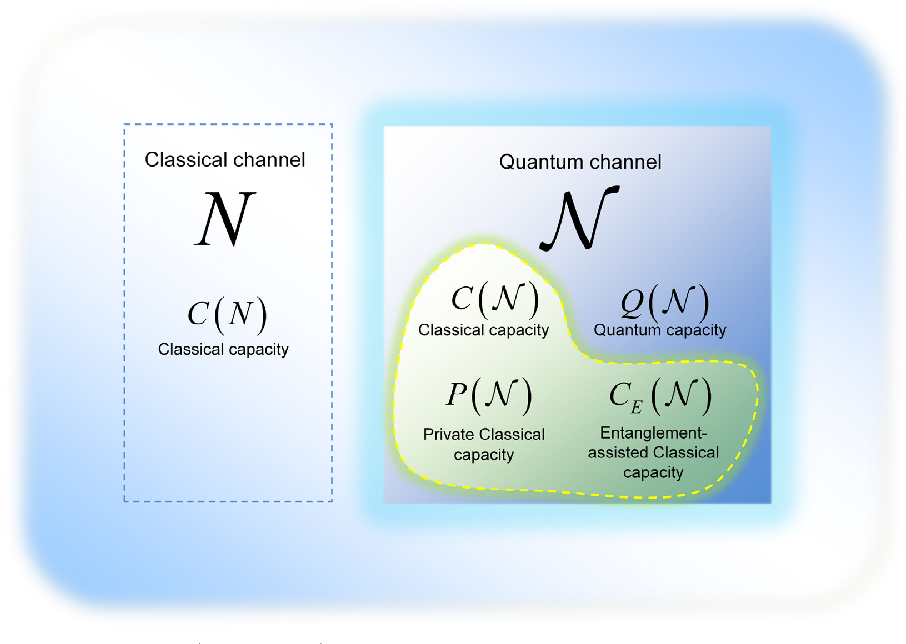
\includegraphics[width=0.75\textwidth]{figures/properties_channels.png}
\end{center}

\textbf{Practical Example:} Consider a noisy quantum channel, such as a fiber optic cable carrying photons. Each photon represents a \textit{quantum state}, which carries the classical information like \textit{0}, \textit{1}, or a \textit{superposiition} of values. In the real world, however, these cables introduce noise. 
\begin{itemize}
    \item \textbf{Photon Loss:} Some photons fail to reach the receiver.
    \item  \textbf{Depolarization:} The state of a photon changes unpredictably.
    \item \textbf{Environmental interference:} Vibrations, temperature changes, or impurities in the fiber can alter the transmitted states.
\end{itemize}

\subsection{Formula for Classical Capacity}
The classical capacity is determined using the Holevo-Schumacher-Westmoreland (HSW) theorem, which relates it to the \textbf{Holevo quantity}. Mathematically, it is given by:
\[
C(\mathcal{N}) = \lim_{n \to \infty} \frac{1}{n} \chi\left(\mathcal{N}^{\otimes n}\right),
\]
where:
\begin{itemize}
    \item \(n\): The number of channel uses.
    \item \(\mathcal{N}^{\otimes n}\): The channel applied in parallel over \(n\) uses.
    \item \(\chi(\mathcal{N})\): The Holevo quantity, an upper bound on the information that can be transmitted.
\end{itemize}

\begin{center}
    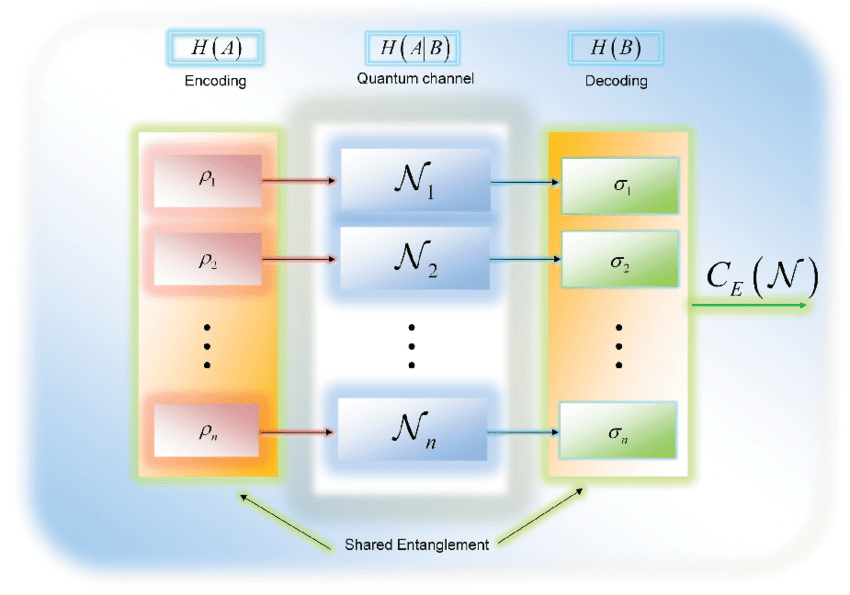
\includegraphics[width=0.75\textwidth]{figures/classical_cap.png}
\end{center}

\subsubsection{The Holevo Quantity}
The Holevo quantity \(\chi\) quantifies the classical information extractable from quantum states. For a quantum channel \(\mathcal{N}\) and a classical ensemble of quantum states \(\{p_i, \rho_i\}\), it is defined as:
\[
\chi(\mathcal{N}, \{p_i, \rho_i\}) = S\left( \sum_i p_i \mathcal{N}(\rho_i) \right) - \sum_i p_i S\left( \mathcal{N}(\rho_i) \right),
\]
where:
\begin{itemize}
    \item \(\{p_i, \rho_i\}\): The ensemble of quantum states \(\rho_i\) sent with probabilities \(p_i\).
    \item \(S(\rho) = -\text{Tr}[\rho \log \rho]\): The von Neumann entropy.
    \item \(\mathcal{N}(\rho_i)\): The output of the quantum channel for input state \(\rho_i\).
\end{itemize}

\subsection{Types of Quantum Channels}
Quantum channels are often noisy, and can degrade the transmitted states. Understanding the noise characteristics is crucial for determining capacity.

\textbf{Common Types of Quantum Channels:}
\begin{itemize}
    \item \textbf{Depolarizing Channel:} Randomly replaces a qubit with a completely mixed state.
    \item \textbf{Dephasing Channel:} Introduces noise that destroys superposition by affecting phase information.
    \item \textbf{Amplitude Damping Channel:} Models energy loss, such as photon leakage in optical fibers.
\end{itemize}

\subsection{Computing Classical Capacity}
Determining \(C(\mathcal{N})\) involves:
\begin{enumerate}
    \item \textbf{Step 1:} Evaluate the Holevo quantity \(\chi(\mathcal{N})\) for a single channel use. This requires finding the optimal input ensemble \(\{p_i, \rho_i\}\) that maximizes \(\chi\).
    \item \textbf{Step 2:} Extend to \(n\)-parallel channel uses, taking advantage of collective strategies to enhance transmission. Regularization over \(n\) ensures the true capacity is approached.
\end{enumerate}

\subsubsection{Special Cases and Examples}
\begin{itemize}
    \item \textbf{Perfect Channel:} For an ideal quantum channel with no noise, the classical capacity equals the Shannon entropy of the input states.
    \item \textbf{Completely Depolarizing Channel:} For a channel that randomizes input states entirely, \(C(\mathcal{N}) = 0\), as no meaningful classical information can be transmitted.
\end{itemize}

\subsubsection{Practical Implications}
\begin{enumerate}
    \item \textbf{Communication Systems:} Quantum channels enable classical data transmission through optical fibers and satellites. Noise mitigation and error correction are essential to maximize capacity.
    \item \textbf{Quantum Cryptography:} Classical capacity helps design secure communication protocols, where channel noise complicates eavesdropping but reduces capacity.
    \item \textbf{Quantum Networks:} Classical capacity optimizes hybrid quantum-classical protocols in distributed systems.
\end{enumerate}

\subsection{Summary}
The classical capacity \(C(\mathcal{N})\) measures the maximum reliable classical information transmission over a quantum channel. While the Holevo quantity provides theoretical limits, practical systems use approximations and error correction to approach these limits.

\subsection{Classical Capacity Citations}
\begin{figure}[h]
    \centering
    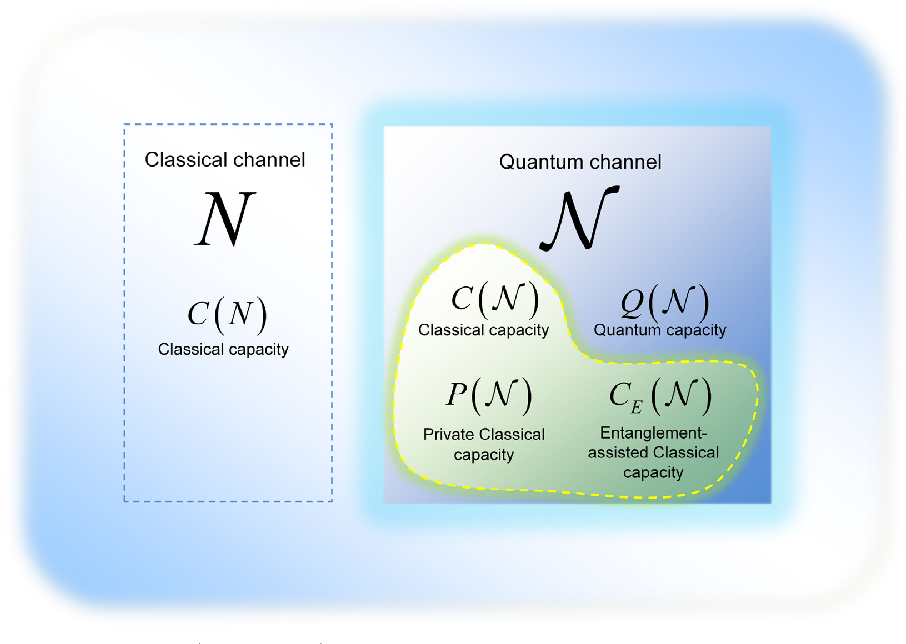
\includegraphics[width=0.75\textwidth]{figures/properties_channels.png}
    \caption{Properties of the Quantum Channel \cite{Gyongyosi2012PropertiesOT}}
\end{figure}

\begin{figure}[h]
    \centering
    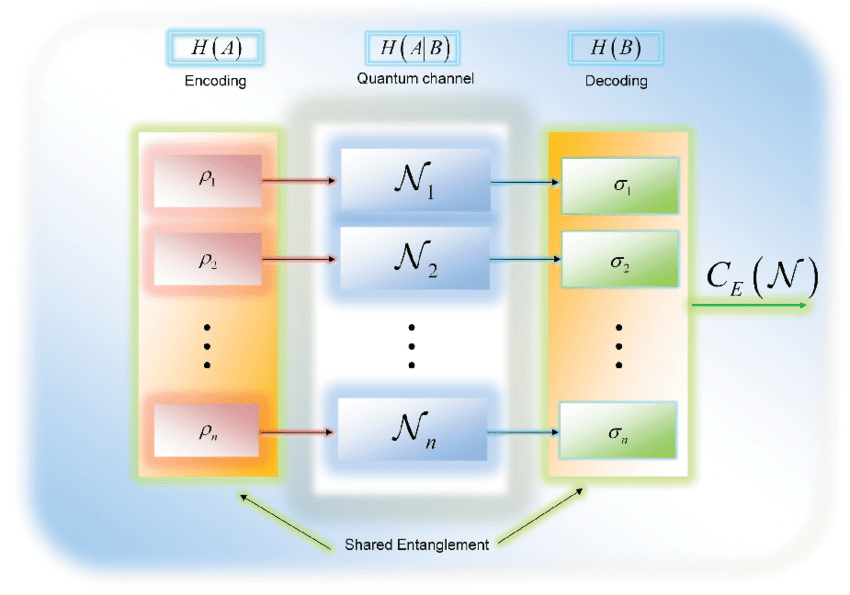
\includegraphics[width=0.75\textwidth]{figures/classical_cap.png}
    \caption{Classical Capacity Illustration \cite{6773024}}
\end{figure}
